\documentclass[class=report, crop=false, 12pt,a4paper]{standalone}
\usepackage{enumitem}
\usepackage{multicol}
\usepackage{graphicx}
\usepackage{float}
\usepackage{amsmath}
\usepackage{amssymb}
\usepackage{mathtools}
\usepackage{siunitx}
\usepackage{commath}
\usepackage{array}
\usepackage{natbib}
\usepackage[a4paper,width=150mm,top=25mm,bottom=25mm]{geometry}
\setlength{\parindent}{0pt}
\begin{document}
\section{Strain energy}
\begin{quotation}
  The energy of a system is the ability of the system to do work.
\end{quotation}
Energy may exist in many forms and can be transformed from one for to another. All forms of energy can be put into two main categories:
\begin{itemize}
  \item Kinetic energy - motion (of waves, electrons, atoms, molecules, substances and objects)
  \item Potential energy - stored energy
\end{itemize}
Strain energy is a form of potential energy that is stored within a material which has been subjected to strain (deformation). If the material remains \textbf{elastic} whilst the deformation is applied, then it is capable of doing an amount of work equal to the stored strain energy when returning to its original dimensions.
\begin{figure}[H]
  \centering
  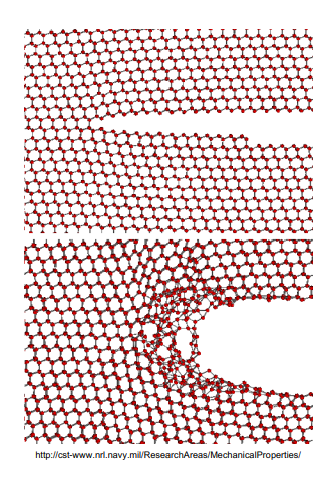
\includegraphics[width = 0.4\textwidth]{../img/diagram8.png}
  \caption{}
\end{figure}
The work done $W$ by the external actions on the structure as effect of the displacements, is equal to the strain energy $U$ stored by internal reaction forces as effect of the deformations within the structure:
\begin{equation}
  W = U
\end{equation}
\begin{figure}[H]
  \centering
  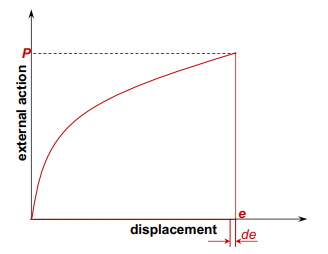
\includegraphics[width = 0.4\textwidth]{../img/diagram9.png}
  \caption{}
\end{figure}
For a gradually applied load, the work done by a force acting on the structure, is given by the area under the force - displacement curve:
\begin{equation}
  W = \int_0^e P \, \dif e
\end{equation}
If displacement is proportional to load (Hookean behaviour)
\begin{equation}
  W = \frac{1}{2} Pe
\end{equation}
\begin{figure}[H]
  \centering
  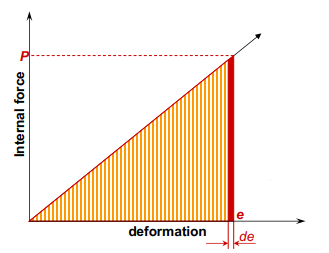
\includegraphics[width = 0.4\textwidth]{../img/diagram10.png}
  \caption{}
\end{figure}
For a gradually applied load, the energy stored by the internal actions into the structure, is given by the area under the internal force - deformation curve:
\begin{equation}
  U = \int_0^e P \, \dif e
\end{equation}
If deformation is proportional to load (Hookean behaviour):
\begin{equation}
  U = \frac{1}{2} P e
\end{equation}
\subsection{Bending moment}
\begin{figure}[H]
  \centering
  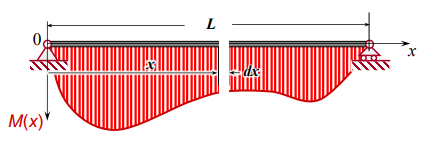
\includegraphics[width = 0.7\textwidth]{../img/diagram11.png}
  \caption{}
\end{figure}
We can determine through various methodologies the distribution of the bending moment. If we want to determine the strain energy at a particular point along the beam, we can extract an elemental portion of the beam with length $\dif x$ from a position $x$ in our coordinate system. This is subjected to a certain bending moment and this will produce a $\dif \theta$ with radius $R$.
\begin{figure}[H]
  \centering
  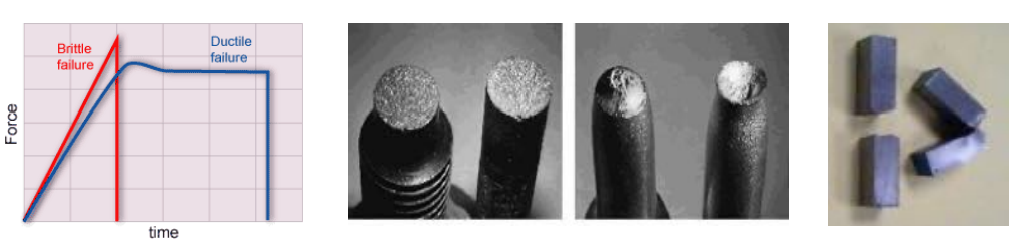
\includegraphics[width = 0.4\textwidth]{../img/diagram12.png}
  \caption{}
\end{figure}
We then know that:
\begin{equation}
  \dif U_M = \frac{1}{2} M \dif \theta
\end{equation}
It is inconvenient to use $\theta$ in our equations and we would like to substitute this for $x$. We know that:
\begin{align}
  \dif \theta = \frac{\dif x}{R} \textrm{ and } \frac{1}{R} = \frac{M}{EI}
\end{align}
(from theory of bending). Therefore:
\begin{equation}
  \dif \theta = \frac{M}{EI} \dif x
\end{equation}
Substituting:
\begin{align}
  \dif U_M = \frac{1}{2} \frac{M^2}{EI} \dif x\\
  U_M = \int_0^L \frac{M^2}{2EI}\, \dif x
\end{align}
\section{Castigliano's Theorem}
Castigliano stated in his engineering thesis that:
\begin{quotation}
  ... the partial derivative of the strain energy, considered as a function of the applied forces acting o na linear elastic structure, with respect to one of these forces, is equal to the displacement in the direction of the force of its point of application.
\end{quotation}
This simply means that if we want to know the displacement from an applied force at the point of application, we can simply take the partial derivative of the strain energy.
\begin{figure}[H]
  \centering
  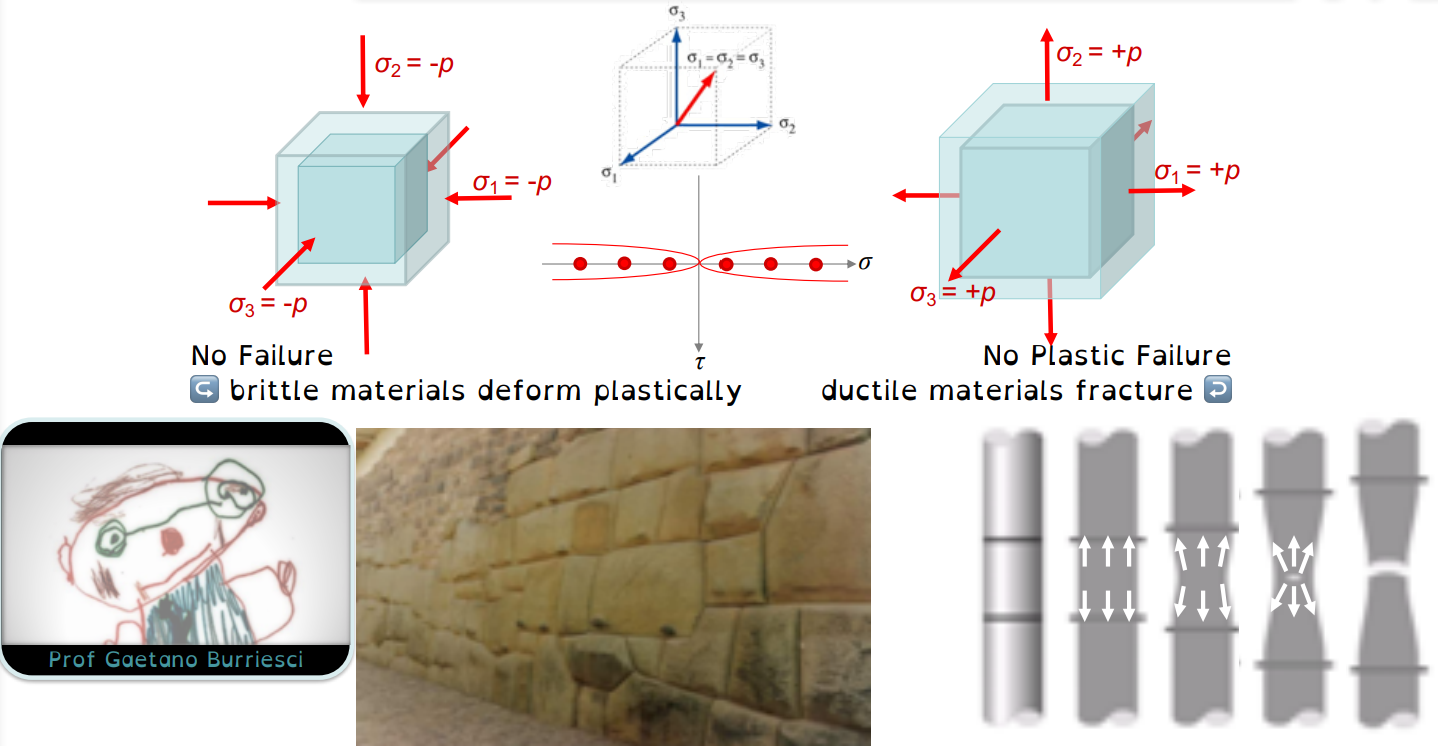
\includegraphics[width = 0.4\textwidth]{../img/diagram13.png}
  \caption{}
\end{figure}
\begin{align}
  \delta_A &= \frac{\partial U}{\partial P_A}, \ \delta_B = \frac{\partial U}{\partial P_B}\\
  \delta_C &= \frac{\partial U}{\partial P_C}, \ \theta_D = \frac{\partial U}{\partial M_D}
\end{align}
In practice, the displacement $\delta_i$ at any load $P_i$ acting upon a system is given by:
\begin{equation}
  \delta_i = \frac{\partial U}{\partial P_i}
\end{equation}
where $U$ is the strain energy of the system due to all loads including $P_i$. The load may be a force, in which case a linear displacement is obtained; or a rotational moment, in which case an angular displacement is obtained. The displacement (linear or angular) will result positive in the same sense as the applied action (force or moment).
\begin{figure}[H]
  \centering
  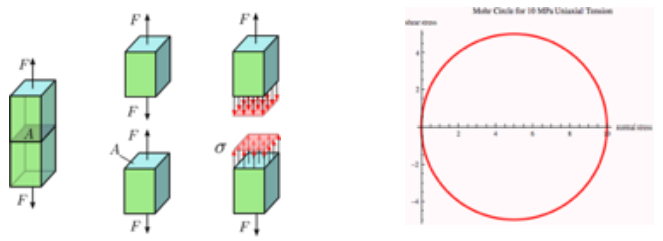
\includegraphics[width = 0.4\textwidth]{../img/diagram14.png}
  \caption{}
\end{figure}
\subsection{Application of Castigliano's theorem}
We know that:
\begin{equation}
  \delta_i = \frac{\partial U_M}{\partial P_i}
\end{equation}
We also know that:
\begin{equation}
  U_M = \int_0^L \frac{M^2}{EI}\, \dif x
\end{equation}
Substituting:
\begin{align}
  \delta_i &= \frac{\partial}{\partial P_i} \int_0^L \frac{M^2}{2EI} \, \dif x\\
  \delta_i &= \int_0^L \frac{\partial}{\partial P_i} \left(\frac{M^2}{2EI}\right) \, \dif x 
\end{align}
An alternative expression using the chain rule can be derived as:
\begin{gather}
  \delta_i = \frac{\partial U_M}{\partial P_i} = \frac{\partial U_M}{\partial M} \cdot \frac{\partial M}{\partial P_i} = \int_0^L \frac{\partial}{\partial M} \left(\frac{M^2}{2EI}\right)\frac{\partial M}{\partial P_i} \, \dif x
\end{gather}
This leads to:
\begin{gather}
  \frac{\partial}{\partial M} \frac{\partial M^2}{2EI} = \frac{M}{EI}\\
  \delta_i = \int_0^L \frac{M}{EI} \frac{\partial M}{\partial P_i}\dif x
\end{gather}
\section{Examples and applications}
\subsection{Dummy loads}
\subsubsection{Example 1}
Determine the deflection of the free end of the beam in the direction of $P$.
\begin{figure}[H]
  \centering
  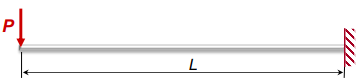
\includegraphics[width = 0.7\textwidth]{../img/diagram15.png}
  \caption{}
\end{figure}
Bending moment:
\begin{equation}
  M = -P x
\end{equation}
Castigliano's theorem:
\begin{gather}
  \delta = \int_0^L \frac{\partial}{\partial P} \left(\frac{M^2}{2EI}\right) \, \dif x = \int_0^L \frac{\partial }{\partial P} \left(\frac{P^2 x^2}{2EI}\right)\, \dif x = \int_0^L \frac{Px^2}{EI} \, \dif x = \frac{PL^3}{3EI}\\
  \delta = \frac{PL^3}{3EI}
\end{gather}
\subsubsection{Example 2}
\begin{figure}[H]
  \centering
  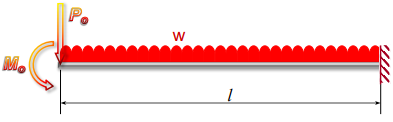
\includegraphics[width = 0.7\textwidth]{../img/diagram16.png}
  \caption{}
\end{figure}
We can utilise dummy loads in order to analyse our system. The bending moment is:
\begin{equation}
  M = - \frac{wx^2}{2} - P_0 x - M_0 
\end{equation}
Castigliano's theorem (alternative equation):
\begin{align}
  \delta = \int_0^L \frac{M}{EI} \frac{\partial M}{\partial P_0} \, \dif x \textrm{ with } \frac{\partial M}{\partial P_0} = \frac{\partial }{\partial P_0} \left(-\frac{wx^2}{2} - P_0 x - M_0\right) = -x
\end{align}
Substituting:
\begin{align}
  \delta = \int_0^L \frac{1}{EI} \left(-\frac{wx^2}{2}\right)\left(-x\right)\, \dif x = \frac{w}{2EI} \int_0^L x^3 \, \dif x = \frac{wL^4}{8EI}
\end{align}
Note: as $P_0 x$ and $M_0$ are dummy loads, they do not need to be included in our final equation for $\delta$.
\subsection{Curved beams}
In many applications beams are curved in the form of circular arcs, rather than straight. Standard formulae used for straight beam deflections cannot be used for curved beams. In this case the application of Castigliano's theorem allows for a solution.
\begin{quotation}
  \textbf{Thin curved beams} are characterised by a beam depth which is small compared to the radius of curvature.
\end{quotation}
As a result:
\begin{itemize}
  \item curvature effects and stress concentration in the cross-section are negligible: stresses are essentially linear like those of a straight beam
  \item effects of normal and shear forces are typically negligible
\end{itemize}
\begin{figure}[H]
  \centering
  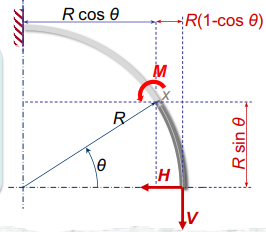
\includegraphics[width = 0.4\textwidth]{../img/diagram17.png}
  \caption{}
\end{figure}
In the case of curved beams, it is more convenient to refer to the angle $\theta$ than to to the beam length. The bending moment can be characterised as:
\begin{itemize}
  \item Contribution to bending moment from horizontal force $H$: $M_H$ = force $\cdot$ distance $ = H\cdot R \sin{\theta}$
  \item Contribution to bending moment from vertical force $V$: $M_V$ = force $\cdot$ distance $ = V\cdot R \left(1-\cos{\theta}\right)$
\end{itemize}
\begin{equation}
  M(\theta) = HR \sin \theta + VR \left(1-\cos\theta\right)
\end{equation}
\end{document}